\chapter{Representations of compact Lie groups}

For finite groups, we defined an inner product of maps:
\[
    \langle F, H \rangle = \frac{1}{|G|} \sum_{g \in G} \overline{F(g)}\, H(g).
\]
For Lie groups the sum is replaced by an integral, $\sum \to \int$. This does not converge in
general, but for compact Lie groups we obtain a well-defined measure:
\[
    \langle F, H \rangle = \int_G \overline{F(g)}\, H(g)\, d\mu.
\]

\section{Integration on manifolds}

\defn{Metric}{
    A \textbf{metric} on $M$ is a family of non-degenerate inner products
    \[
        g_m : T_m M \otimes T_m M \to \mathbb{R}
    \]
    for $m \in M$, depending smoothly on $m \in M$. Smooth in this context means in local
    coordinates
    \[
        g(x)\Big( v^i \frac{\partial}{\partial x^i},\, w^j \frac{\partial}{\partial x^j} \Big)
            = \sum_{i,j} g(x)_{ij}\, v^i w^j
    \]
    with the $g(x)_{ij}$ being smooth functions of $x$. A metric is called \textbf{Euclidean} if it
    is positive definite at each point.
    \index{metric}\index{metric!Euclidean}
}

An integral is defined by
\[
    \int_M f\, d\mathrm{vol}(g).
\]
In local coordinates,
\[
    \int_U f(x^i)\, \sqrt{\det\big(g(x^i)\big)}\,
        \underbrace{dx^1 \cdots dx^n}_{\text{Lebesgue measure on } U \subseteq \mathbb{R}^n}.
\]

To extend this to all of $M$ we need to cover $M$. There are two options:
\begin{itemize}
    \item Cover $M$ with a collection of charts and use a partition of unity. Let
    $\{U_i\}_{i \in I}$ be a cover. A \textbf{partition of unity} is a collection of functions
    $f^i : M \to \mathbb{R}$ such that each $f^i$ is $0$ outside $U^i$ and $\sum_i f^i = 1$. Then
    \[
        \int_M f\, d\mathrm{vol}(g) = \sum_i \int f^i\, f\, \sqrt{\det\big(g(x^i)\big)}\, dx^1 \cdots dx^n.
    \]
    This makes sure to eliminate over-counting.
    \index{partition of unity}

    \item More practical: find charts such that the complement is of lower dimension, hence of
    measure $0$.
\end{itemize}

\ex{
    \begin{itemize}
        \item The circle $S^1$:
        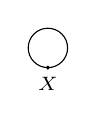
\begin{tikzpicture}[baseline=-2pt, scale=0.5]
            \draw (0,0) circle (0.5);
            \filldraw (0,-0.5) circle (1pt);
            \node[below, font=\scriptsize] at (0,-0.5) {$X$};
        \end{tikzpicture}
        removing a point gives a chart $S^1 \setminus \{X\} \xrightarrow[\theta]{\sim} (0, 2\pi) \subset \mathbb{R}$.
        Since $X$ is lower-dimensional, it does not matter whether we include it or not, and
        \[
            \int_{S^1} f\, d\mathrm{vol}(g) = \int_0^{2\pi} f(\theta)\, \sqrt{g(\theta)}\, d\theta.
        \]
        \item The three-sphere $S^3 \cong \mathrm{SU}(2)$:
        \[
            \int_{S^3} f\, d\mathrm{vol}(g)
                = \int_0^{2\pi}\!\!\int_0^{\pi}\!\!\int_0^{\pi}
                    f(\theta, \phi, \chi)\, \sqrt{\det\big(g(\theta, \phi, \chi)\big)}\,
                    d\theta\, d\phi\, d\chi.
        \]
    \end{itemize}
}

This is for a general manifold. But we need metrics that are compatible with the group structure.

\defn{Left- and right-invariant metric}{
    Let $G$ be a Lie group and $m$ a metric on $G$. We say $m$ is \textbf{left invariant} if
    \[
        m_h\big(V_h, V_h'\big) = m_{g \cdot h}\big((l_g)_* V_h,\, (l_g)_* V_h'\big),
    \]
    where $(l_g)_*$ is the pushforward (differential) of left multiplication $l_g : x \mapsto g \cdot x$.
    It is \textbf{right invariant} if the same holds for right multiplication.
    \index{metric!left invariant}\index{metric!right invariant}
}

Equivalently, for a left-invariant metric the integral is left-invariant:
\[
    \int_G l_g^* f\, d\mathrm{vol}(m) = \int_G f\, d\mathrm{vol}(m),
\]
where $l_g^* f = f \circ l_g$ is the pullback along left multiplication. For a left-invariant metric
we furthermore have
\[
    m_g\big(V_g, V_g'\big) = m_e\big((l_{g^{-1}})_* V_g,\, (l_{g^{-1}})_* V_g'\big),
    \qquad (*)
\]
so a left-invariant metric is determined by its value at the identity,
\[
    m_e : \mathfrak{g} \otimes \mathfrak{g} \to \mathbb{R}.
\]
On the other hand, $(*)$ can be used to define a left-invariant metric from an inner product on
$\mathfrak{g}$.

If $G$ is compact, then
\[
    \int_G 1\, d\mathrm{vol}(m) < \infty,
\]
and hence we can normalize $m$ such that
\[
    \int_G 1\, d\mathrm{vol}(m) = 1.
\]

\thm{Haar measure}{
    There exists a unique left-invariant (normalized) measure on $G$. It is called the \textbf{Haar
    measure} $d\mu$. For compact $G$ it is also right invariant.
    \index{Haar measure}\index{measure!Haar measure}
}

\rmkb{
    A general topological space is compact if for every cover $\{U_i\}_{i \in I}$ there exists a
    finite subcover. For submanifolds of $\mathbb{R}^n$ this is equivalent to being closed and
    bounded.
}

\ex{
    \begin{itemize}
        \item $U(1) = \{ e^{i\phi} \in \mathbb{C} \mid \phi \in [0, 2\pi) \}$, with Haar measure
        \[
            d\mu = \frac{1}{2\pi}\, d\phi.
        \]
        \item Via the exponential map $\exp : \mathfrak{g} \to G$: for $\mathrm{SU}(2)$,
        \[
            g(\phi, \theta, \psi) := \exp\!\Big( \frac{i\phi}{2\pi}\, \sigma_3 \Big)
                \exp\!\Big( \frac{i\theta}{2\pi}\, \sigma_2 \Big)
                \exp\!\Big( \frac{i\psi}{2\pi}\, \sigma_1 \Big),
        \]
        with $\phi \in [0, 2\pi)$, $\theta \in [0, \pi)$, $\psi \in [0, 4\pi)$, and Haar measure
        \[
            d\mu = \frac{1}{16\pi^2}\, \sin(\theta)\, d\phi\, d\theta\, d\psi.
        \]
        \item $\mathrm{GL}(n)$ (non-compact), with left-invariant measure
        \[
            d\mu = |\det \gamma|^{-n} \prod_{i,j} d E_{ij}.
        \]
    \end{itemize}
}

\thmp{Weyl's unitarity trick}{\index{Weyl's unitarity trick}\index{unitarity trick}
    Let $G$ be a compact Lie group and $(V, \rho)$ a finite-dimensional complex representation.
    \begin{itemize}
        \item $V$ admits a $G$-invariant scalar product.
        \item $V$ is completely reducible, i.e. for a subrepresentation $V_1 \subseteq V$ there
        exists $V_2 \subseteq V$ such that $V_1 \oplus V_2 \cong V$ as $G$-representations.
    \end{itemize}
}{
    Let $\langle -, - \rangle : \overline{V} \otimes V \to \mathbb{C}$ be a scalar product on $V$.
    Define
    \[
        \langle v, w \rangle_G := \int_G \big\langle \rho(g) v,\, \rho(g) w \big\rangle\, d\mu.
    \]
    This is $G$-invariant. For a subrepresentation $V_1 \subseteq V$ we set
    $V_2 = V_1^{\perp}$ (the orthogonal complement with respect to $\langle -, - \rangle_G$), so that
    \[
        V_1 \oplus V_2 = V.
    \]
    (See Maschke's theorem, \ref{thm:maschke}.)
}

\rmkb{
    \begin{itemize}
        \item Every $\mathrm{SU}(2)$ representation can be made unitary. Hence the corresponding
        $\mathfrak{sl}(2)$-representation is unitary, so $H$ acts by a self-adjoint operator and is
        therefore diagonalizable in such a finite-dimensional representation.
        \item Each simple Lie algebra $\mathfrak{g}$ has a real form such that the corresponding Lie
        group is compact; it is characterized by the Killing form $\kappa(-,-)$ being negative
        definite on it. Hence each finite-dimensional representation of $\mathfrak{g}$ is completely
        reducible.
    \end{itemize}
}

\defn{Character}{
    Let $(V, \rho)$ be a representation of a compact Lie group $G$. The \textbf{character} of $V$ is
    the function
    \[
        \chi_V : G \to \mathbb{C}, \qquad g \mapsto \mathrm{tr}_V\big(\rho(g)\big).
    \]
    \index{character}
}

\rmkb{
    The characters satisfy:
    \begin{itemize}
        \item $\chi_V(h g h^{-1}) = \chi_V(g)$, hence $\chi_V$ is a class function:
        \[
            \chi_V \in \mathrm{Cl}(G) := \big\{ f \in L^2(G) \mid f(h g h^{-1}) = f(g) \big\}.
        \]
        \item A finite-dimensional representation is fully determined by its character.
        \item $\chi_{V \otimes W}(g) = \chi_V(g)\, \chi_W(g)$.
        \item $\chi_{V \oplus W}(g) = \chi_V(g) + \chi_W(g)$.
    \end{itemize}
    \index{class function}\index{character!class function}
}

\ex{
    \begin{itemize}
        \item \textbf{$\mathrm{U}(1)$.} Since $\mathrm{U}(1)$ is abelian, its irreducible
        representations are $1$-dimensional, and they correspond to Lie group homomorphisms
        $\mathrm{U}(1) \to \mathrm{U}(1)$. What are all smooth such homomorphisms? By Lie's first
        theorem they are completely characterized by Lie algebra maps $\mathbb{R} \xrightarrow{\,\cdot\, a\,} \mathbb{R}$;
        but $\mathrm{U}(1)$ is not simply connected, so we must ask whether the map descends:
        \begin{center}
        \begin{tikzcd}[row sep=2.4em, column sep=3.2em, ampersand replacement=\&]
            \mathbb{R} \arrow[d] \arrow[dr] \& \\
            \mathrm{U}(1) \arrow[r, dashed] \& \mathrm{U}(1)
        \end{tikzcd}
        \end{center}
        Here the vertical arrow is the covering map $x \mapsto e^{ix}$, the diagonal arrow is
        $x \mapsto \exp(ixa)$, and the dashed arrow is the sought homomorphism
        $\mathrm{U}(1) \to \mathrm{U}(1)$. Such a homomorphism exists if and only if
        \[
            a \cdot (x + 2\pi) = a \cdot x \bmod 2\pi
            \quad\Longleftrightarrow\quad
            a \in \mathbb{Z}.
        \]
        Hence all irreducible $\mathrm{U}(1)$-representations are labelled by $\mathbb{Z}$, with
        characters
        \[
            \chi_a\big(e^{ix}\big) = e^{ixa}.
        \]

        \item \textbf{$\mathrm{SU}(2)$.} Representations are labelled by a non-negative integer $k$
        (the highest weight). The conjugacy classes are represented by
        \[
            \begin{pmatrix} e^{i\theta} & 0 \\ 0 & e^{-i\theta} \end{pmatrix}
            = \exp(i\theta H), \qquad H = \begin{pmatrix} 1 & 0 \\ 0 & -1 \end{pmatrix},
            \qquad \theta \in [0, \pi).
        \]
        From the earlier $\mathfrak{sl}(2)$ computation,
        \[
            \chi_{V_k}(\theta) = \frac{\sin\big((k+1)\theta\big)}{\sin(\theta)}.
        \]
        For a class function $f \in \mathrm{Cl}(\mathrm{SU}(2))$, integration reduces to (a special
        case of the \emph{Weyl integration formula})
        \[
            \int_{\mathrm{SU}(2)} f\, d\mu = \frac{2}{\pi} \int_0^{\pi} f(\theta)\, \sin^2(\theta)\, d\theta.
        \]
        In particular the characters are orthonormal:
        \[
            \langle \chi_{V_k}, \chi_{V_{k'}} \rangle
                = \int_{g \in \mathrm{SU}(2)} \overline{\chi_{V_k}}\, \chi_{V_{k'}}(g)\, d\mu
                = \frac{2}{\pi} \int_0^{\pi} \sin\big((k+1)\theta\big) \sin\big((k'+1)\theta\big)\, d\theta
                = \delta_{k, k'}.
        \]
    \end{itemize}
}

\thm{}{
    Let $G$ be a compact Lie group. The characters $\chi_V$ for all irreducible finite-dimensional
    representations of $G$ form an orthonormal \emph{Hilbert basis} with respect to
    \[
        \langle F, H \rangle = \int_G \overline{F(g)}\, H(g)\, d\mu.
    \]
    (Without proof.)
    \index{Hilbert basis}\index{character!orthonormality}
}

\rmkb{
    Hilbert basis: it is not necessary that an element is a finite sum of basis elements, but there
    always exists a convergent expansion in the basis.
}

\ex{
    For $\mathrm{SU}(2)$, $V_2 \otimes V_1 \cong V_3 \oplus V_1$. We showed this before using the
    weights; now again with characters. We have
    \[
        \chi_{V_2 \otimes V_1}(\theta) = \frac{\sin(3\theta)\, \sin(2\theta)}{\sin(\theta)^2},
    \]
    and hence, using $\sin(2\theta) = 2\sin(\theta)\cos(\theta)$ and
    $\sin(3\theta)\cos(\theta) = \tfrac{1}{2}\big(\sin(4\theta) + \sin(2\theta)\big)$,
    \begin{align*}
        \big\langle \chi_{V_k},\, \chi_{V_2 \otimes V_1} \big\rangle
            &= \frac{2}{\pi} \int_0^{\pi} \frac{\sin\big((k+1)\theta\big)\, \sin(3\theta)\, \sin(2\theta)}{\sin(\theta)}\, d\theta \\
            &= \frac{4}{\pi} \int_0^{\pi} \sin\big((k+1)\theta\big)\, \sin(3\theta)\, \cos(\theta)\, d\theta \\
            &= \frac{2}{\pi} \int_0^{\pi} \Big( \sin\big((k+1)\theta\big)\sin(4\theta)
                + \sin\big((k+1)\theta\big)\sin(2\theta) \Big)\, d\theta \\
            &= \delta_{3,k} + \delta_{1,k}.
    \end{align*}
    This confirms $V_2 \otimes V_1 \cong V_3 \oplus V_1$.
}

A torus can be written as $\mathbb{T}^n = \mathrm{U}(1)^{\times n}$.

\defn{Maximal torus}{
    For a simple Lie group $G$, a \textbf{maximal torus} is an abelian subgroup $H \leq G$ which is
    isomorphic to $\mathbb{T}^n$ and maximal with this property. The corresponding
    $\mathfrak{h} \subseteq \mathfrak{g}$ is a Cartan subalgebra (after complexification
    $\otimes\, \mathbb{C}$).
    \index{torus!maximal torus}\index{maximal torus}
}

\rmkb{
    The space of conjugacy classes of $G$ is isomorphic to $H/W$, the maximal torus modulo the Weyl
    group. For $\mathrm{SU}(2)$ we found $\mathrm{U}(1)/\mathbb{Z}_2$.
}

\ex{
    \emph{(Fourier transform.)} A class function on $\mathrm{U}(1)$ is a function
    $f : \mathrm{U}(1) \to \mathbb{C}$, equivalently a function $f : \mathbb{R} \to \mathbb{C}$ with
    $f(x + 2\pi) = f(x)$. With
    \[
        \chi_k(x) = e^{ikx},
    \]
    we recover the Fourier series
    \[
        f(x) = \sum_{k \in \mathbb{Z}} \langle \chi_k, f \rangle\, e^{ikx},
        \qquad
        \langle \chi_k, f \rangle = \frac{1}{2\pi} \int_0^{2\pi} e^{-ikx}\, f(x)\, dx.
    \]
}

What about $L^2(G)$? Yes, this leads to the \emph{non-abelian Fourier transform}. For each
irreducible representation $(V, \rho)$ of $G$ we fix a basis $e_1, \dots, e_n$ with $n = \dim V$. In
this basis
\[
    \rho(g) = \big\{ \rho(g)_{ij} \big\}_{i,j = 1, \dots, n}.
\]

\defn{Matrix coefficient functions}{
    The functions $\rho(g)_{ij} : G \to \mathbb{C}$ are called \textbf{matrix coefficient functions}.
    \index{matrix coefficient function}
}

\thm{Peter--Weyl theorem}{
    The matrix coefficient functions, multiplied by $\frac{1}{\sqrt{n}}$, form an orthonormal basis
    of $L^2(G)$.
    \index{Peter-Weyl theorem}
}

\rmkb{
    There is a map
    \begin{align*}
        V^* \otimes V &\to L^2(G), \\
        f \otimes v &\mapsto \big( g \mapsto f(\rho^V(g)\, v) \big).
    \end{align*}
    In this formulation, the Peter--Weyl theorem says that
    \[
        \bigoplus_{V \text{ irrep.}} V^* \otimes V \to L^2(G)
    \]
    is a Hilbert space isomorphism. Explicitly, any (square-integrable) function $f : G \to \mathbb{C}$
    can be written as
    \[
        f(g) = \sum_V \sum_{i,j = 1}^{\dim(V)} \hat{f}(V, i, j)\, \rho^V_{ij}(g),
    \]
    with
    \[
        \hat{f}(V, i, j) = \int_{g \in G} \dim(V)^{-\frac{1}{2}}\, \overline{\rho^V_{ij}(g)}\, f(g)\, d\mu.
    \]
}

\rmkb{
    This is useful for solving PDEs, e.g. the heat equation. We pick a bi-invariant metric on $G$
    (e.g. $-\kappa$ extended to $G$) and form the Laplacian
    \[
        \Delta f(x) = \underbrace{m^{ij}\, \frac{\partial}{\partial x^i} \frac{\partial}{\partial x^j}\, f(x)}_{\Delta},
        \qquad
        \Delta : L^2(G) \to L^2(G), \quad \Delta u = -\operatorname{div}\big(\operatorname{grad}(u)\big).
    \]
    The heat equation reads
    \[
        \frac{\partial}{\partial t}\, u(t, g) + \Delta\, u(t, g) = 0.
    \]
    The action $G \curvearrowright L^2(G)$ differentiates to $\mathfrak{g} \curvearrowright L^2(G)$
    (``$X \triangleright f = \frac{\partial}{\partial x} f(g)$''), and $\Delta$ acts as the Casimir
    $C_2$, which acts by multiplication. Hence
    \[
        \partial_t\, u(t, g) = -C_2\, u(t, g), \qquad u : G \to \mathbb{C}.
    \]
    On $V_\Lambda$ we have $C_2 v = (\Lambda, \Lambda + 2\rho)\, v$ for $v \in V_\Lambda$, so the
    equation has solutions
    \[
        u^{ij}_{V_\Lambda}(t, g) = e^{-t\, (\Lambda, \Lambda + 2\rho)}\, \rho^{V_\Lambda}_{ij}(g).
    \]
    For an arbitrary initial condition
    $u_0(g) = \sum_{\Lambda, i, j} \tilde{u}_0(\Lambda, i, j)\, \rho^{V_\Lambda}_{ij}(g)$, the solution
    is
    \[
        u(t, g) = \sum_{\Lambda, i, j} \tilde{u}_0(\Lambda, i, j)\, e^{-t\, (\Lambda, \Lambda + 2\rho)}\, \rho^{V_\Lambda}_{ij}(g).
    \]
}

\ex{
    \textbf{$2$-dimensional Yang--Mills theory} with gauge group $G$ a compact Lie group, on a closed
    surface (for instance a genus-$2$ surface).

    \emph{Canonical quantization.} To each spatial slice $S^1$ we assign a Hilbert space. The
    classical configuration space is the moduli space of flat $G$-connections on $S^1$ modulo gauge
    transformations,
    \[
        \mathrm{Bun}_G^{\nabla}(S^1) / \text{Gauge} \cong G / G,
    \]
    the adjoint quotient of $G$ by conjugation. Hence
    \[
        \mathcal{H} = ``L^2\big(\mathcal{F}(S^1)\big)" = L^2(G/G) \cong \mathrm{Cl}(G),
    \]
    the space of class functions.

    \emph{Hamiltonian.} The Hamiltonian is proportional to the quadratic Casimir,
    \[
        \mathbb{H} : \mathcal{H} \to \mathcal{H}, \qquad \mathbb{H} = \frac{e^2}{2}\, C_2,
    \]
    with $e$ the coupling constant. By the character theory above it acts diagonally: on the
    irreducible character $\chi_{V_\Lambda}$ it acts by the scalar
    $\frac{e^2}{2}(\Lambda, \Lambda + 2\rho)$.

    \emph{Discretization.} Triangulate the surface and assign a group element $g_E \in G$ to each
    edge $E$. To each triangle $\triangle$ of area $a$, with boundary holonomy
    $g_2^{-1} g_3^{-1} g_1$,
    \begin{center}
    \begin{tikzpicture}[>=Stealth, scale=1.1]
        \coordinate (A) at (0,0);
        \coordinate (B) at (2,0);
        \coordinate (C) at (1,1.5);
        \draw[->] (A) -- (B) node[midway, below] {$g_1$};
        \draw[->] (A) -- (C) node[midway, left] {$g_2$};
        \draw[->] (B) -- (C) node[midway, right] {$g_3$};
    \end{tikzpicture}
    \end{center}
    we assign the heat kernel, and integrate over all edges with the Haar measure:
    \[
        Z = \int_{G^{|E|}} \prod_{\triangle} \bigg( \sum_V \dim(V)\, e^{-C_2(V)\, a}\,
            \chi_V\big(g_2^{-1} g_3^{-1} g_1\big) \bigg)\, d\mu.
    \]
    This is independent of the chosen triangulation, so the continuum limit is well defined.
}

\emph{(The remainder of this section situates the example in its topological context and goes
slightly beyond the board sketch.)}

Gluing the triangles over a closed orientable surface $\Sigma_g$ of genus $g$ and total area
$A = \sum_{\triangle} a$, triangulation independence collapses the lattice integral to a single sum
over irreducible representations,
\[
    Z(\Sigma_g) = \sum_V (\dim V)^{2 - 2g}\, e^{-\frac{e^2 A}{2}\, C_2(V)},
\]
where $2 - 2g = \chi(\Sigma_g)$ is the Euler characteristic \cite{WittenQuantumGaugeTheoriesTwoDimensions1991}.
This is pure representation theory: the ingredients $\dim V$ and $C_2(V)$ are exactly the
Peter--Weyl and character data of $G$. In the zero-area (topological) limit $A \to 0$ the
exponential drops out and
\[
    Z(\Sigma_g) = \sum_V (\dim V)^{2 - 2g}
\]
becomes a topological invariant of $\Sigma_g$ --- the partition function of a $2$-dimensional
topological quantum field theory.

\thm{2-dimensional TQFTs and Frobenius algebras}{
    A $2$-dimensional topological quantum field theory is a symmetric monoidal functor
    $Z : 2\mathrm{Cob} \to \mathrm{Vect}_{\mathbb{C}}$ out of the category $2\mathrm{Cob}$ of
    $2$-dimensional cobordisms. Such functors are equivalent to commutative Frobenius algebras: the
    object $Z(S^1)$ carries a natural commutative Frobenius algebra structure, and this assignment is
    an equivalence of categories \cite{KockFrobeniusAlgebras2DTQFT2004}.
    \index{topological quantum field theory}\index{Frobenius algebra}
}

For $2$-dimensional Yang--Mills the relevant Frobenius algebra is precisely
$Z(S^1) = \mathrm{Cl}(G)$, the class functions, with convolution as multiplication and the
$L^2$-pairing $\langle F, H \rangle = \int_G \overline{F(g)}\, H(g)\, d\mu$ as the Frobenius form. The
genus-$g$ invariant $\sum_V (\dim V)^{2-2g}$ is its associated cobordism invariant, and this is the
point at which category theory --- the category $2\mathrm{Cob}$ --- enters explicitly.

\rmkb{
    Specializing $G$ to a \emph{finite} group reproduces (untwisted) Dijkgraaf--Witten theory with
    gauge group $G$: the same class-function / Frobenius-algebra structure now counts $G$-bundles on
    $\Sigma_g$ weighted by their automorphisms. Its three-dimensional counterpart is governed by the
    quantum double (Drinfeld double) $D(G)$, whose braided category of representations has as simple
    objects the \emph{anyons} underlying topological quantum computing
    \cite{KitaevFaultTolerantAnyons2003}. This is where the categorical machinery is genuinely
    headed; see also \cite{MullerSchweigertGNSDijkgraafWitten2018} for a construction of
    three-dimensional abelian Dijkgraaf--Witten theories.
}
